\documentclass[12pt, oneside]{article}     

% packages
\usepackage[margin=1in]{geometry}                  	
\geometry{letterpaper}                   	
\usepackage{graphicx}				
\usepackage{amssymb}
\usepackage{amsmath}                                                                                                                                                                                                                                                                                                                                                                                                                                                                                                                                                                                          
\usepackage{bm}
\usepackage{float}
\usepackage[nodisplayskipstretch]{setspace}
\usepackage{enumitem}
\usepackage{fancyheadings}
\usepackage{mathtools}
\usepackage{csquotes}
\usepackage{hanging}

% Configuration
\setstretch{1.5}
\pagestyle{fancy}
\input{"../middle_header.txt"}
\chead{Multilevel Model Building}
\title{\vspace{-1cm}Multilevel Model Building}

% Custom commands
\newif\ifanswers
 \answerstrue % comment out to hide answers

\begin{document}
\maketitle

\thispagestyle{fancy}

\section*{Objectives}
This lab exercise has two parts---a model \emph{building} exercise and a model \emph{coding} exercise.  For some there are likely \emph{more} problems than time available for completion. The material covered here is important and broadly useful, and it will be worthwhile for you to pursue what you do not finish after the course. The problem and answer format should allow you to make progress on your own. We suggest that you go back and forth between the model writing exercises (herein) and the coding exercises (provided as \texttt{MultilevelModelCoding.html}). This exercise will reinforce the following:

\begin{itemize}
\item Diagraming and writing hierarchical models.
\item Using data to ``model parameters.''
\item JAGS coding.
\item Creating index variables, a critically important and useful skill.
\item Use of the multivariate normal distribution to represent random variables that covary.
\end{itemize}

\newpage

\section*{Nitrous oxide emissions from agricultural soils}

Ecological data are often collected at multiple scales or levels of organization in nested designs. ``Group'' is a catchall term for the upper level in many different types of nested hierarchies. Groups could logically be composed of populations, locations, species, treatments, life stages, and individual studies, or really, any sensible category. We have measurements within groups on individual organisms, plots, species, time periods, and so on. We may also have measurements on the groups themselves, that is covariates that apply at the upper level of organization or spatial scale or the category that contains the measurements. Multilevel models represent the way that a quantity of interest responds to the combined influence of observations taken at the group level and within the group. 

Nitrous oxide, a greenhouse gas roughly 300 times more potent than carbon dioxide in forcing atmospheric warming, is emitted when synthetic nitrogenous fertilizers are added to soils. Qian and colleagues (2010) conducted a Bayesian meta-analysis of such additions (gN $\cdot$ ha\textsuperscript{-1}$\cdot$ d\textsuperscript{-1}) using data from a study conducted by Carey (2007), who reviewed 164 relevant studies. Studies occurred at different locations, forming a group-level hierarchy\footnote{We will use only sites that have both nitrogen and carbon data, which reduces the number of sites to 107 in the analysis here.}. Soil carbon content (g $\cdot$ organic C $\cdot$ g\textsuperscript{-1} soil dry matter) was measured as a group-level covariate and is assumed to be measured without error. Observations of $N\textsubscript{2}O$ emission is also assumed to be measured without error and were paired with measurements of fertilizer addition (kgN$\cdot$ ha\textsuperscript{-1}). The effect of different types of fertilizer was also studied. 

\begin{enumerate} [leftmargin=*] 
\item Begin by ignoring the data on soil carbon, site, and fertilizer type. Draw a Bayesian network and write out the posterior and joint distribution for a linear regression model of $N\textsubscript{2}O$ emission on fertilizer addition for a single observation. Use a linearized power function for your deterministic model of emissions. For now, you may use the generic $[\,]$ so that you do not need to write specific distributions. Use $\sigma^{2}$ to represent the uncertainty in your model realizing, of course, that you might need moment matching when you choose a specific distribution.

\ifanswers
\begin{center}
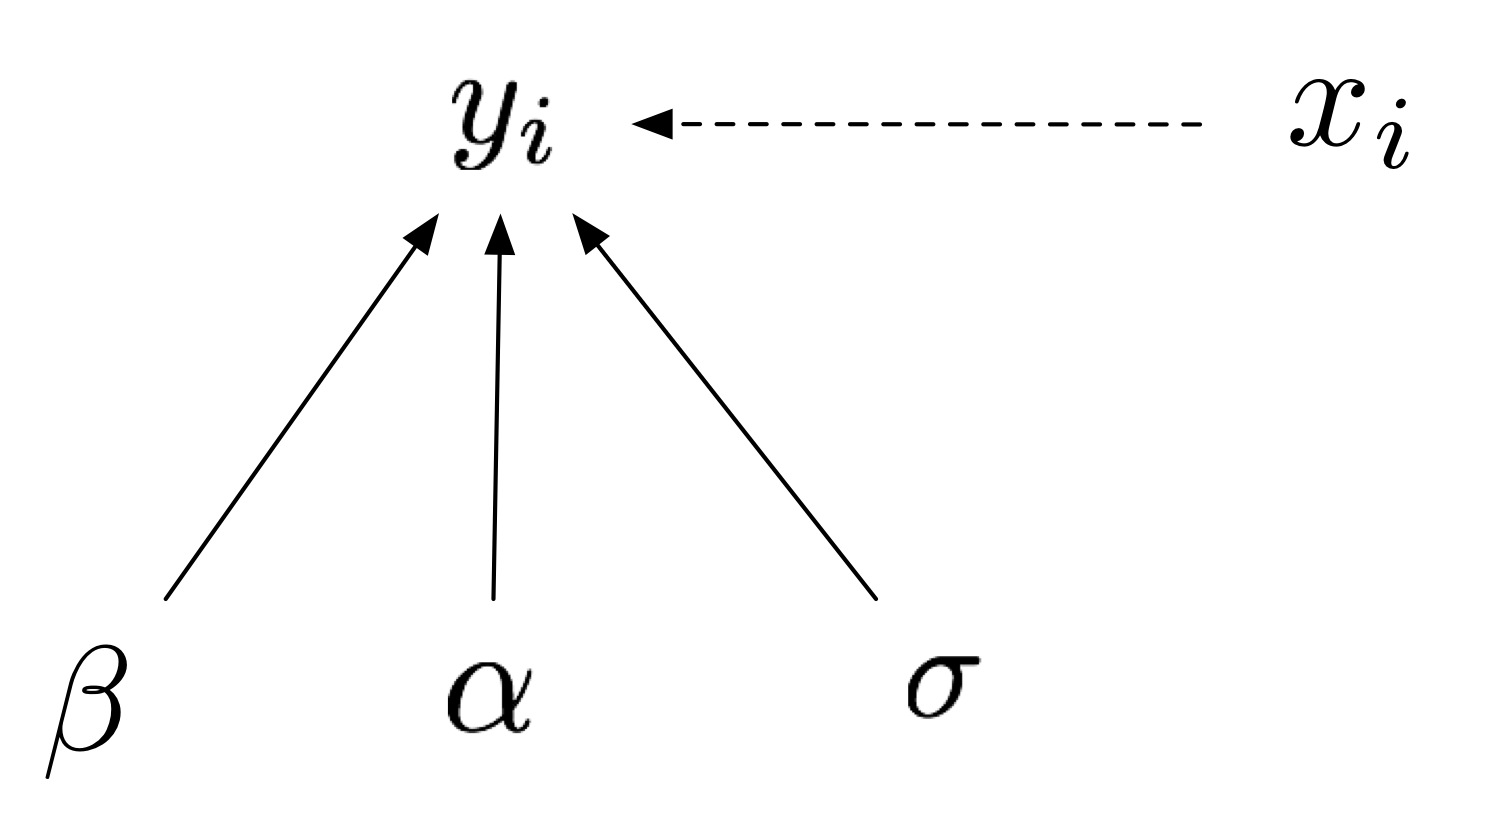
\includegraphics[scale=.5]{DAG1.png}
\end{center}
\begin{eqnarray*}
\mu_{i} & = & \gamma x^{\beta}\\
\alpha & = & \log\big(\gamma\big)\\
\log\big(\mu_{i}\big) & = & \alpha+\beta\log\big(x_{i}\big)\\
g\big(\alpha,\beta,x_{i}\big) & = & \alpha+\beta\log\big(x_{i}\big)\\
\big[\alpha,\beta,\sigma \mid y_{i}\big] & \propto & \big[\log(y_{i})\mid g\big(\alpha,\beta,x_{i}\big),\sigma^{2}\big][\alpha]\big[\beta\big]\big[\sigma \big]\label{eq:mean model for N02 intecept-3}
\end{eqnarray*}	
\fi

\newpage

\item Now treat the intercept in your model as a group level effect (aka, random effect). The model of the process now becomes a linearized power function for your deterministic model of emissions but two subscripts are required, $i$ indexes the measurement within sites and $j$ indexes site. Write the Bayesian model for a single observation using $ij$ notation. Again, using $[\,]$ notation for distributions.  

\ifanswers
\newpage
\begin{center}
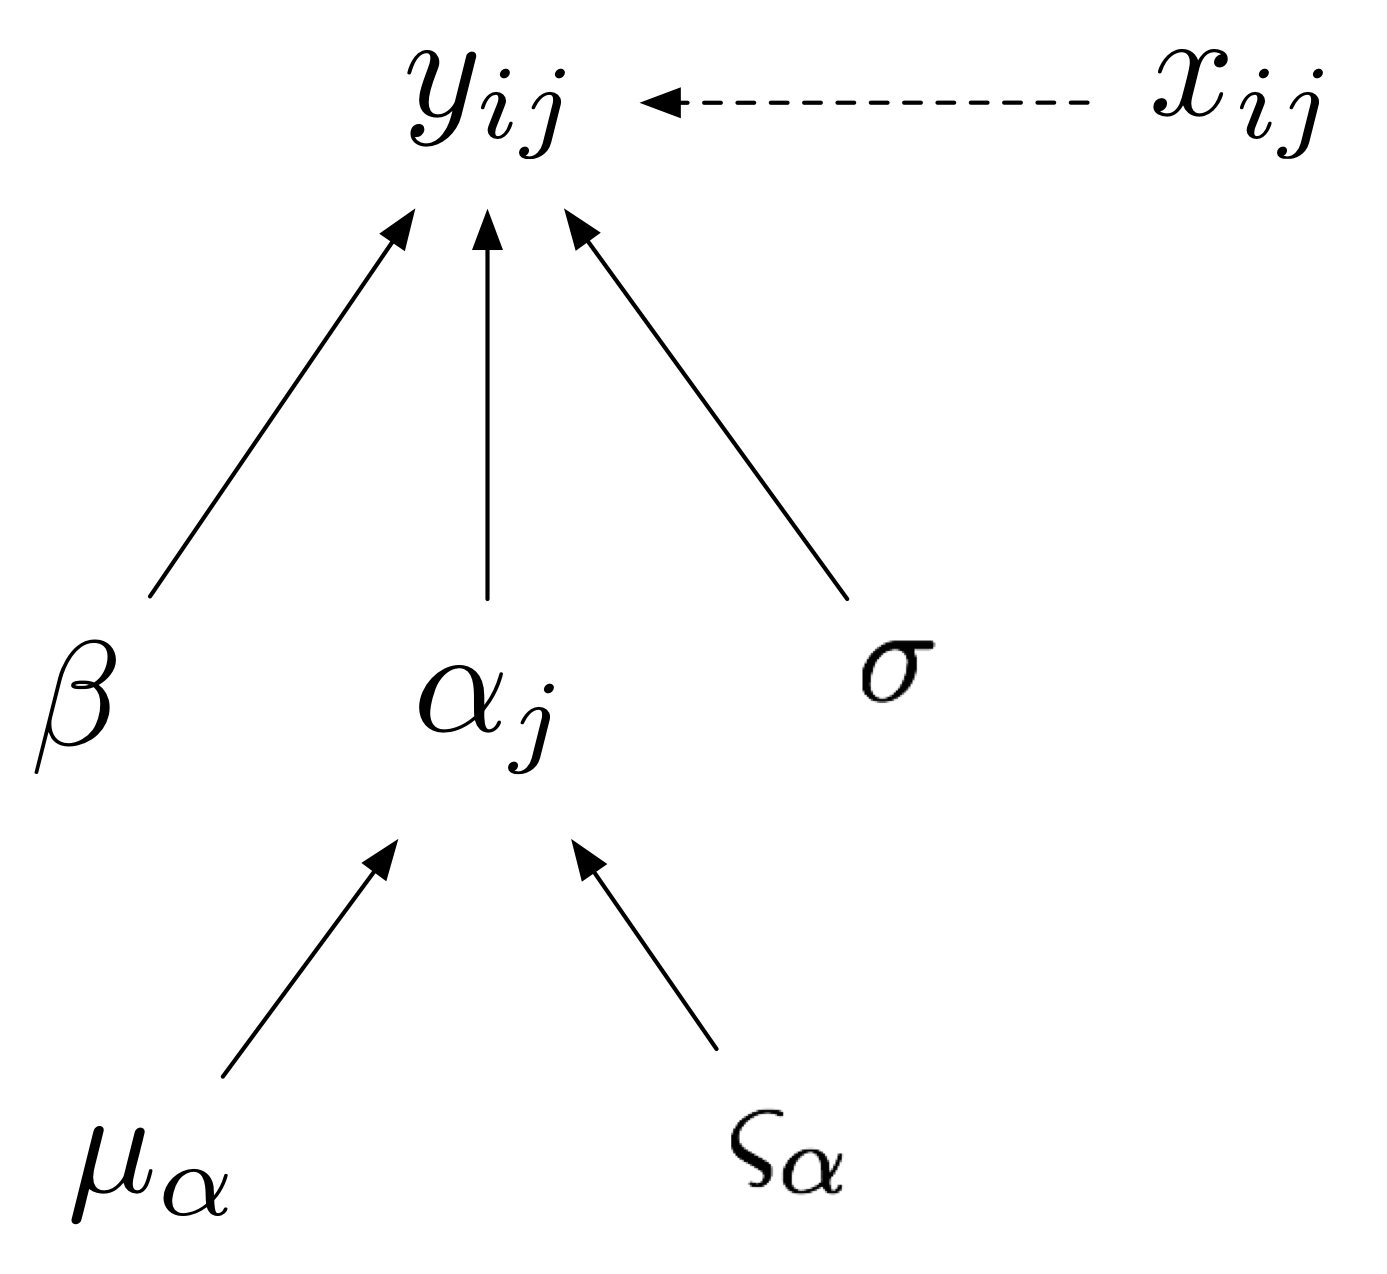
\includegraphics[scale=.5]{DAG2.png}
\end{center}

\begin{eqnarray*}
g\big(\alpha_{j},\beta,x_{ij}\big)&=& \alpha_{j}+\beta\log\big(x_{ij}\big)\\
\big[\alpha_{j},\beta,\mu_{\alpha},\sigma,\varsigma_{\alpha}\mid y_{ij}\big] & \propto & \big[\log(y_{ij})\mid g\big(\alpha_{j},\beta,x_{ij}\big),\sigma^{2}\big]\big[\alpha_{j}\mid\mu_{\alpha},\varsigma_{\alpha}^{2}\big]\big[\beta\big]\big[\sigma\big]\big[\mu_{\alpha}\big]\big[\varsigma_{\alpha}\big]\label{eq:mean model for N02 intecept}
\end{eqnarray*}

where $y_{ij}$ is the $i^{th}$ observation of $N\textsubscript{2}O$ emissions in study $j$; $x_{ij}$ is a paired measurement of fertilizer addition and $\beta$ is the change in $N\textsubscript{2}O$ emissions per unit change in fertilizer addition. The model $g\big(\alpha_{j},\beta,x_{ij}\big)$ represents the hypothesis that the log of emissions increases in direct proportion to the log of fertilizer additions and that this increase is the same for all sites and fertilizer types\footnote{We will remedy this brave assumption later.}. The intercept $\alpha_{j}$ varies among studies as a random variable drawn from a distribution with parameters\footnote{Again, these parameters will \emph{not} be means and variances for any distributions except the normal and Poisson, but it turns out for this example, they are because we will use normals. Remember moment matching for other distributions.} $\mu_{\alpha}$ and $\varsigma_{\alpha}^{2}$. The fact that we explicitly represent variation among studies using the distribution of the $\alpha_{j}$ is what sets this analysis apart from conventional, single level regression that could be done separately for each of the individual sites or by pooling all of the data across sites to estimate a single intercept and slope. The $\sigma^{2}$ represents the uncertainty about $N\textsubscript{2}O$ emissions\footnote{We could have estimated separate $\sigma$ for each site, but this was not done by Carey (2007) and I wanted to maintain consistency with their analysis as much as possible.} and the $\varsigma_{\alpha}^{2}$ represents the uncertainty that arises as a result of variation among sites.$ $   
\fi

\newpage
\item In the previous example, we assumed that there was variation the intercept that was attributable to spatial variation among sites. We did not try to explain that variation, we simply acknowledged that it exists. Now we are going to "model a parameter'' using data at the group-level to explain variation in the intercepts among sites. Modify the previous model to represent the effect of soil carbon on the intercept using the deterministic model. Draw a Bayesian network and write out the posterior and joint distributions for the full dataset, which means you must include the proper products. Use $ij$ notation. You will need to notate that there are $n_{j}$ measurements of {$N\textsubscript{2}O$ emissions paired with fertilizer additions} from study $j$. Chose appropriate distributions for each random variable.

\ifanswers
\newpage
\begin{center}
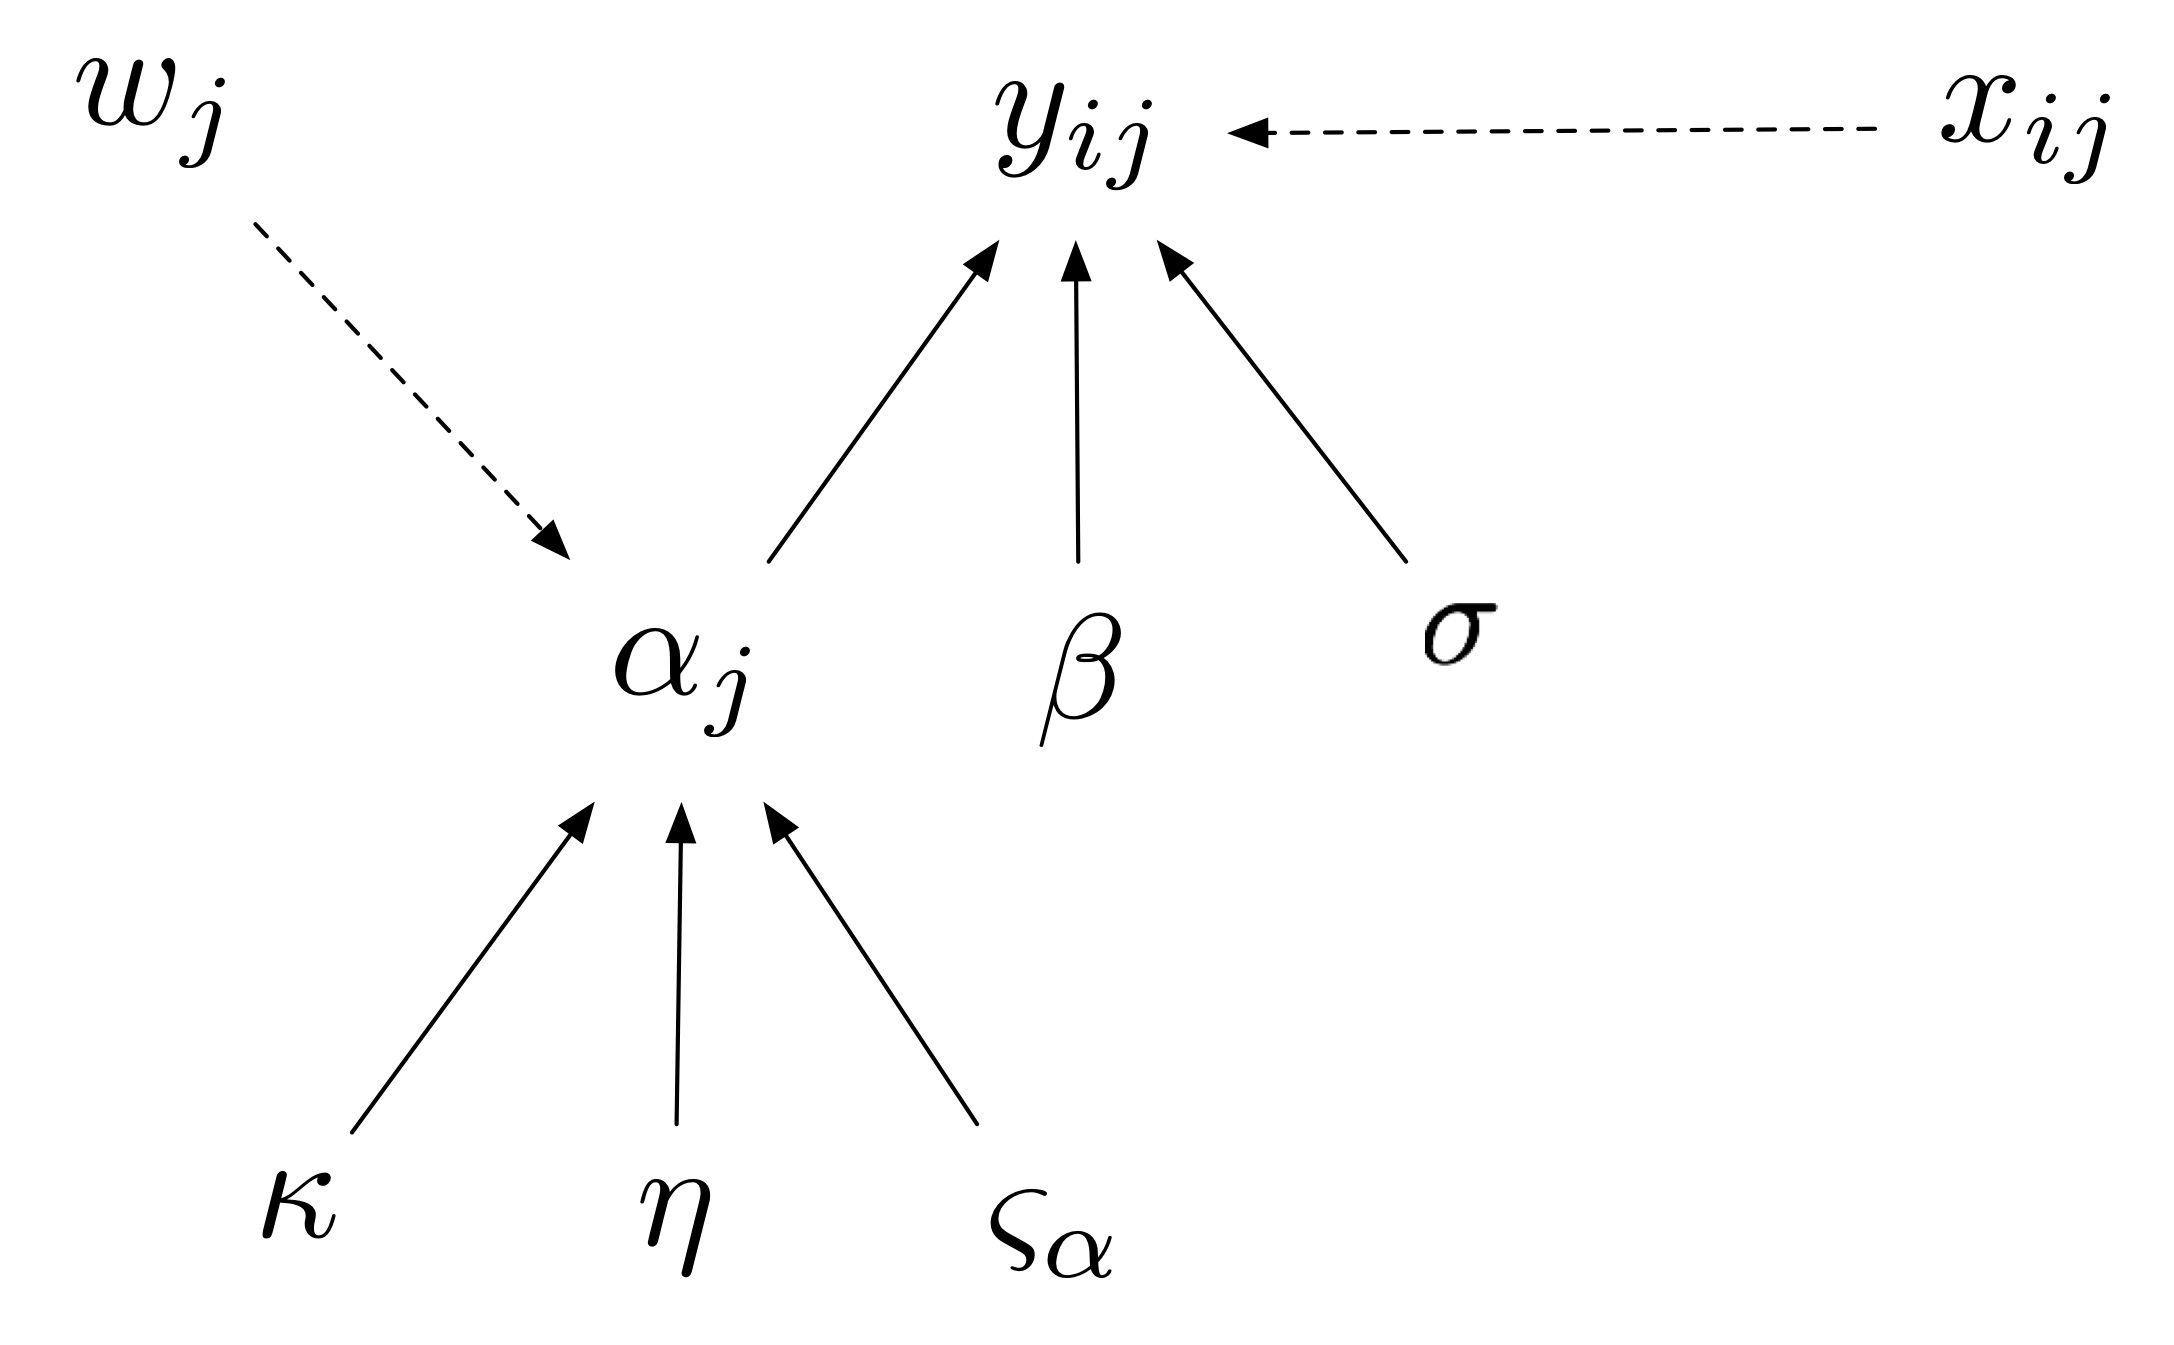
\includegraphics[scale=.5]{DAG3.png}
\end{center}
\begin{align*}
g_{1}\big(\alpha_{j},\beta,x_{ij}\big)  &=\alpha_{j}+\beta\log\big(x_{ij}\big)\\
g_{2}\big(\kappa,\eta,w_{j}\big) &= \kappa+\eta\text{logit}\big(w_{j}\big)\\
\big[\bm{\alpha},\beta,\sigma,\varsigma_{\alpha},\kappa,\eta\mid\mathbf{y}\big] &\propto \prod_{j=1}^{J}\prod_{i=1}^{n_{j}}\text{normal}\big(\log(y_{ij}\big)\mid g_{1}\big(\alpha_{j},\beta,x_{ij}\big),\sigma^{2}\big)\label{eq:mean model for N02 intecept-1}\\
 &\times \text{normal}\big(\alpha_{j}\mid g_{2}\big(\kappa,\eta,w_{j}\big),\varsigma_{\alpha}^{2}\big)\\
 &\times \text{normal}\big(\beta \mid 0,1000\big)\\
 &\times \text{normal}\big(\eta \mid 0,1000\big)\\
 &\times \text{normal}\big(\kappa \mid 0,1000\big)\\
 &\times \text{uniform}\big(\sigma \mid 0,200\big)\\
 &\times \text{uniform}\big(\varsigma_{\alpha} \mid 0,200\big)\\
\end{align*}
\fi

\newpage 

\item Now we are interested in the effect of carbon \emph{and }fertilizer type on $N\textsubscript{2}O$ emissions. Model the effect of carbon as above, but include a group level effect of fertilizer type on the slope of the emission vs fertilizer addition model. This is to say that the slopes of the regressions are drawn from a distribution of fertilizer types. Index plot with $i$, site with $j$, and fertilizer type with $k$. Thus, there will be $K$ slopes, one for each fertilizer
type, drawn from a distribution with mean $\mu_{\beta}$ and variance $\varsigma_{\beta}^{2}$. Modify the carbon model you built in the previous step to incorporate effect of fertilizer type.  

\ifanswers
\newpage
\begin{center}
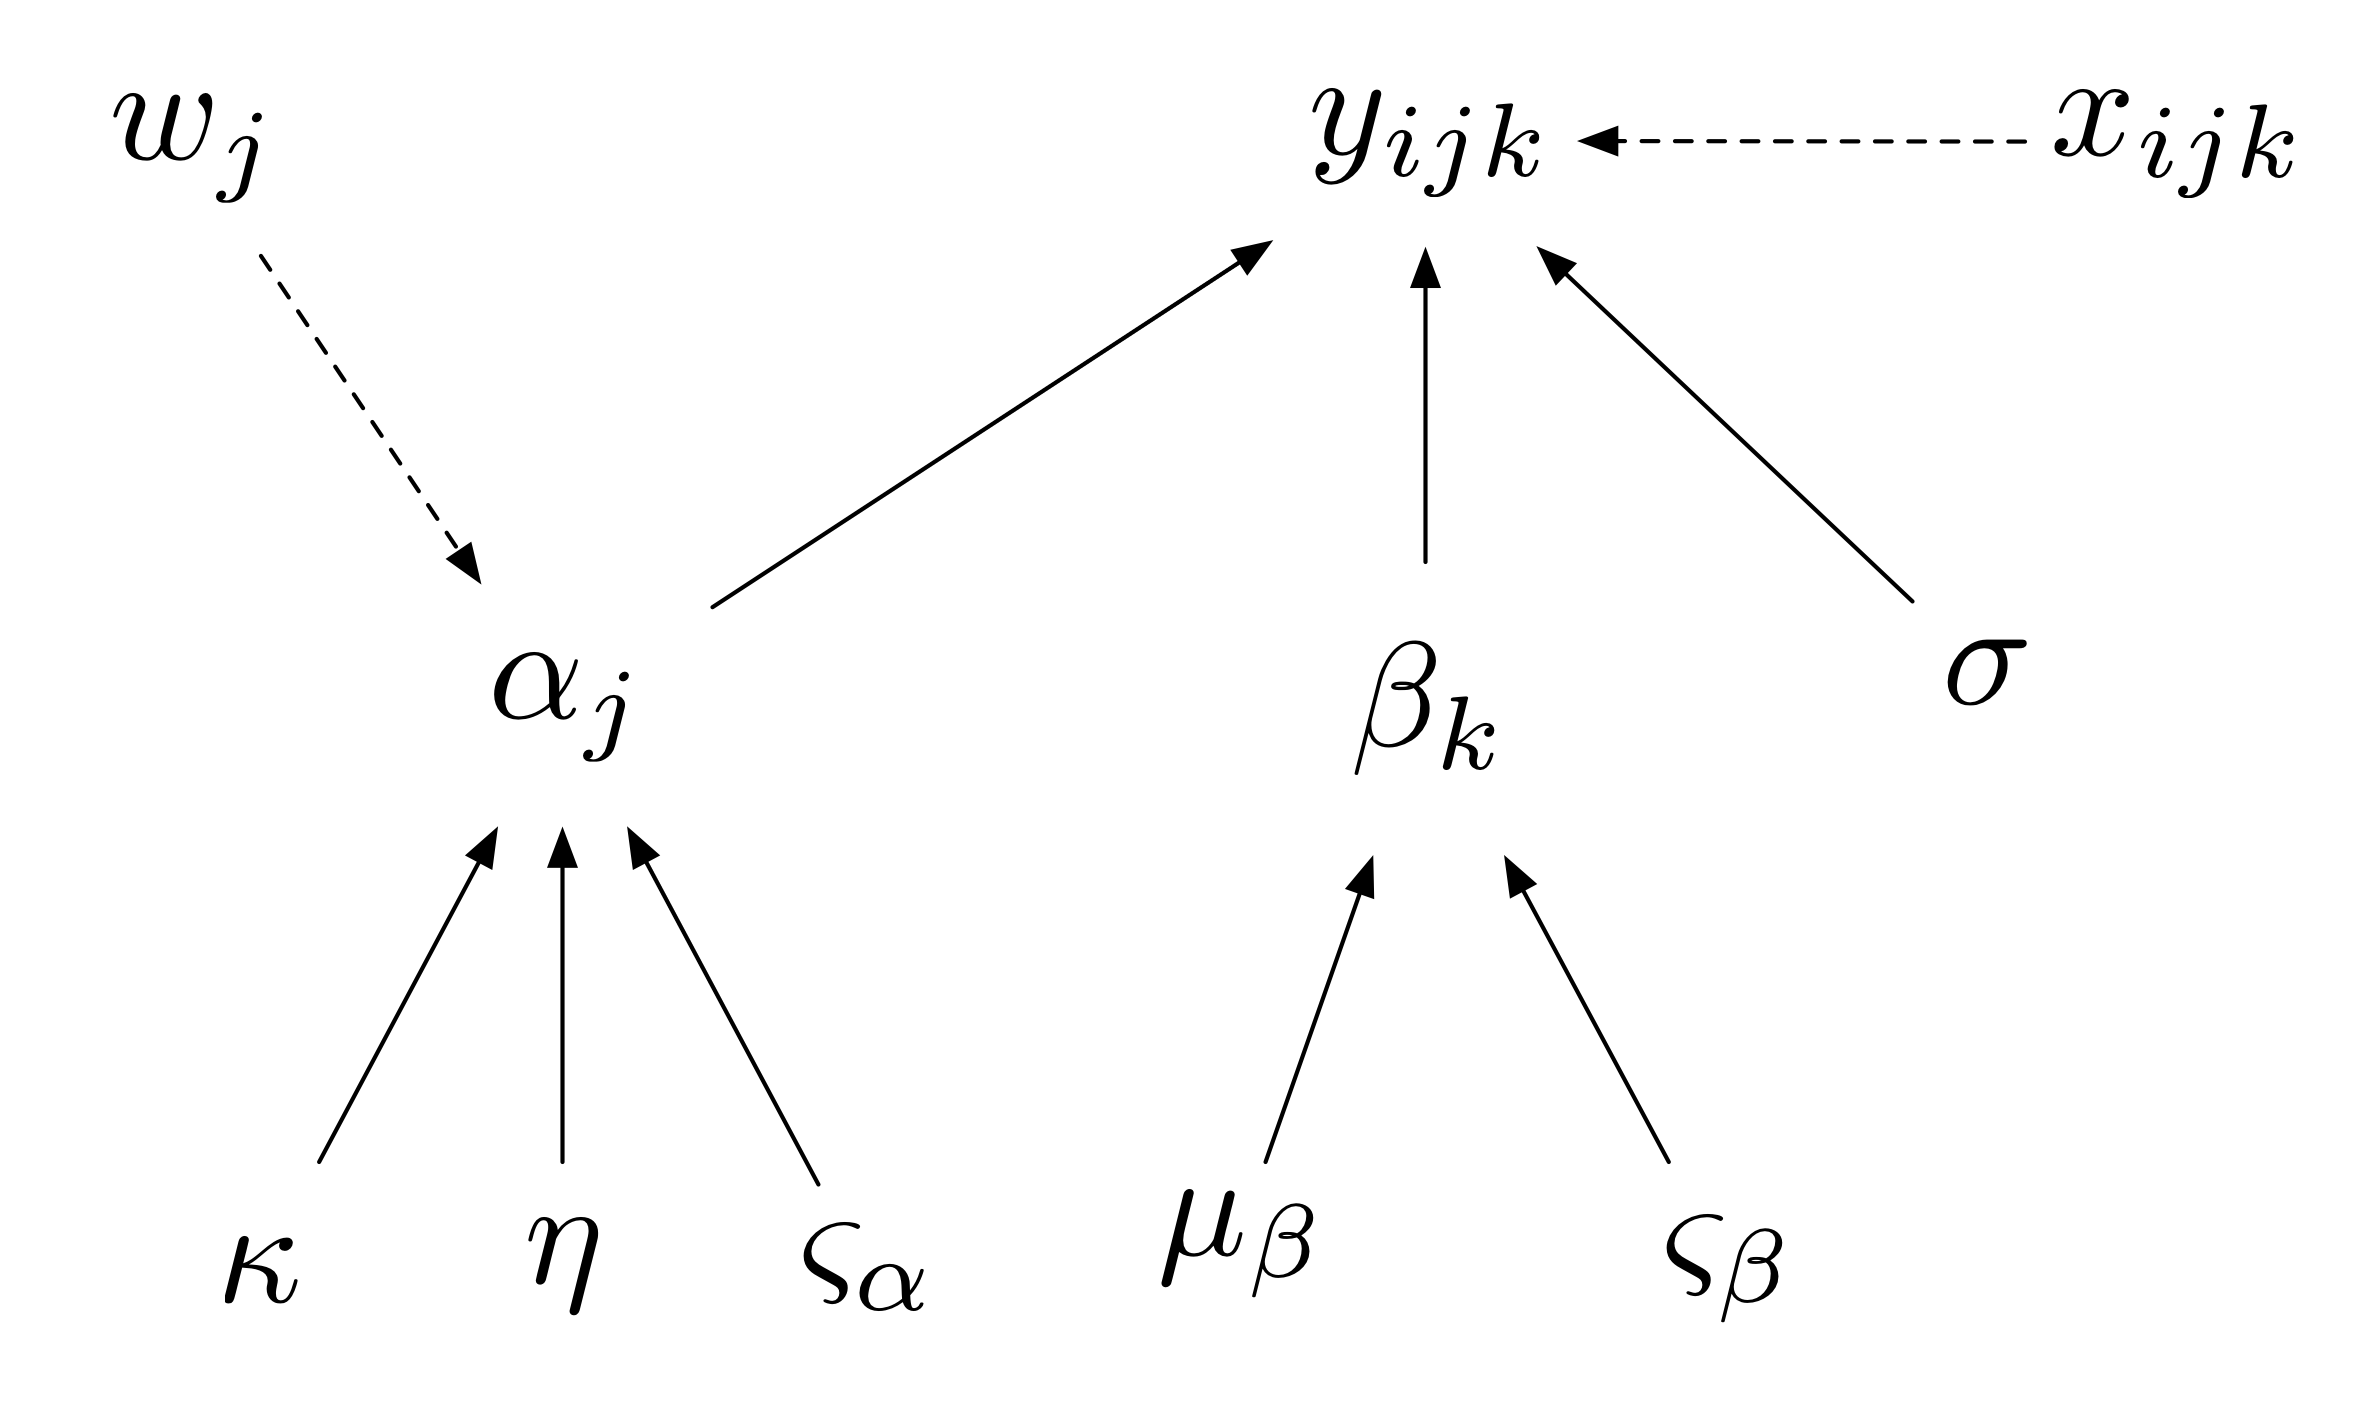
\includegraphics[scale=.5]{DAG4.png}
\end{center}
\begin{align*}
g_{1}\big(\alpha_{j},\beta_{k},x_{ijk}\big) &= \alpha_{j}+\beta_{k}\log(x_{ijk})\\
g_{2}\big(\kappa,\eta,w_{j}\big) &= \kappa+\eta\text{logit}(w_{j})\\
\big[\bm{\alpha},\bm{\beta},\sigma,\varsigma_{\alpha},\kappa,\eta,\mu_{\beta,}\varsigma_{\beta}\mid\mathbf{y}\big] &\propto \prod_{j=1}^{J}\prod_{k=1}^{K_{j}}\prod_{i=1}^{n_{j}}\text{normal}\big(\log\big(y_{ijk}\big)\mid
g_{1}\big(\alpha_{j},\beta_{k},x_{ijk}\big),\sigma^{2}\big)\\
 & \times \text{normal}\big(\alpha_{j}\mid g_{2}\big(\kappa,\eta,w_{j}\big),\varsigma_{\alpha}^{2}\big)\\
 & \times \text{normal}\big(\beta_{k}\mid \mu_{\beta},\varsigma_{\beta}^{2}\big)\\
 & \times \text{normal}\big(\eta\mid 0,1000\big)\\
 & \times \text{normal}\big(\kappa\mid 0,1000\big)\\
 & \times \text{uniform}\big(\sigma\mid 0,100\big)\\
 & \times \text{uniform}\big(\varsigma_{\alpha}\mid 0,200\big)\\
 & \times \text{normal}\big(\mu_{\beta}\mid 0,1000\big)\\
 & \times \text{uniform}\big(\varsigma_{\beta}\mid 0,200\big)
\end{align*}
\fi

\newpage

\item Now return to problem 2 where you assumed that different groups had the different intercepts but the same slope, which is to say that individual sites had emission responses to fertilizer that were parallel. This seems unreasonable (particularly when you look at lattice plots of the data), representing the need to model group effects on intercepts \emph{and slopes.} The idea is that both the slope and the intercept are random variables drawn from a distribution of slopes and intercepts where variation in the values of the random variable is attributable to unspecified spatial differences among sites. It is tempting to simply add a distribution for the slopes
in the same way you modeled the intercepts, and you will see papers where this is done (wrongly). However, when you seek to understand group effects on multiple parameters you must account for the way that the parameters \emph{covary}. Write a model for group effects on slope \emph{and} intercepts. Exploit the following hints.

\begin{itemize}
\item Represent the slope and intercept as a two element vector for each group and use a multivariate normal distribution in the same way you used a normal for the intercept. So the individual slopes ($\alpha_{j})$ and intercept ($\beta_{j})$ will be drawn from 

\begin{equation*}
\left(\begin{array}{c}
\alpha_{j}\\
\beta_{j}
\end{array}\right)\sim\text{multivariate normal}\left(\left(\begin{array}{c}
\mu_{\alpha}\\
\mu_{\beta}
\end{array}\right),\bm{\Sigma}\right)
\end{equation*}
\vspace{5mm}

\item The second parameter in the multivariate normal is a variance-covariance matrix representing how the slope and intercept covary. It has variance terms on the diagonal, and covariance terms on the off-diagonal, i.e., 

\begin{equation*}
\bm{\Sigma}=\left(\begin{array}{cc}
\varsigma_{\alpha}^{2} & \text{Cov}(\bm{\alpha},\bm{\beta})\\
\text{Cov}(\bm{\alpha},\bm{\beta}) & \varsigma_{\beta}^{2}
\end{array}\right).
\end{equation*}
\vspace{5mm}

The covariance terms are defined as $\text{Cov}(\bm{\alpha},\bm{\beta})=\rho\varsigma_{\alpha}\varsigma_{\beta}$ where $\rho$ is the coefficient of correlation between $\bm{\alpha}$ and $\bm{\beta}$.
\end{itemize}
\end{enumerate}

\ifanswers
\newpage
\begin{center}
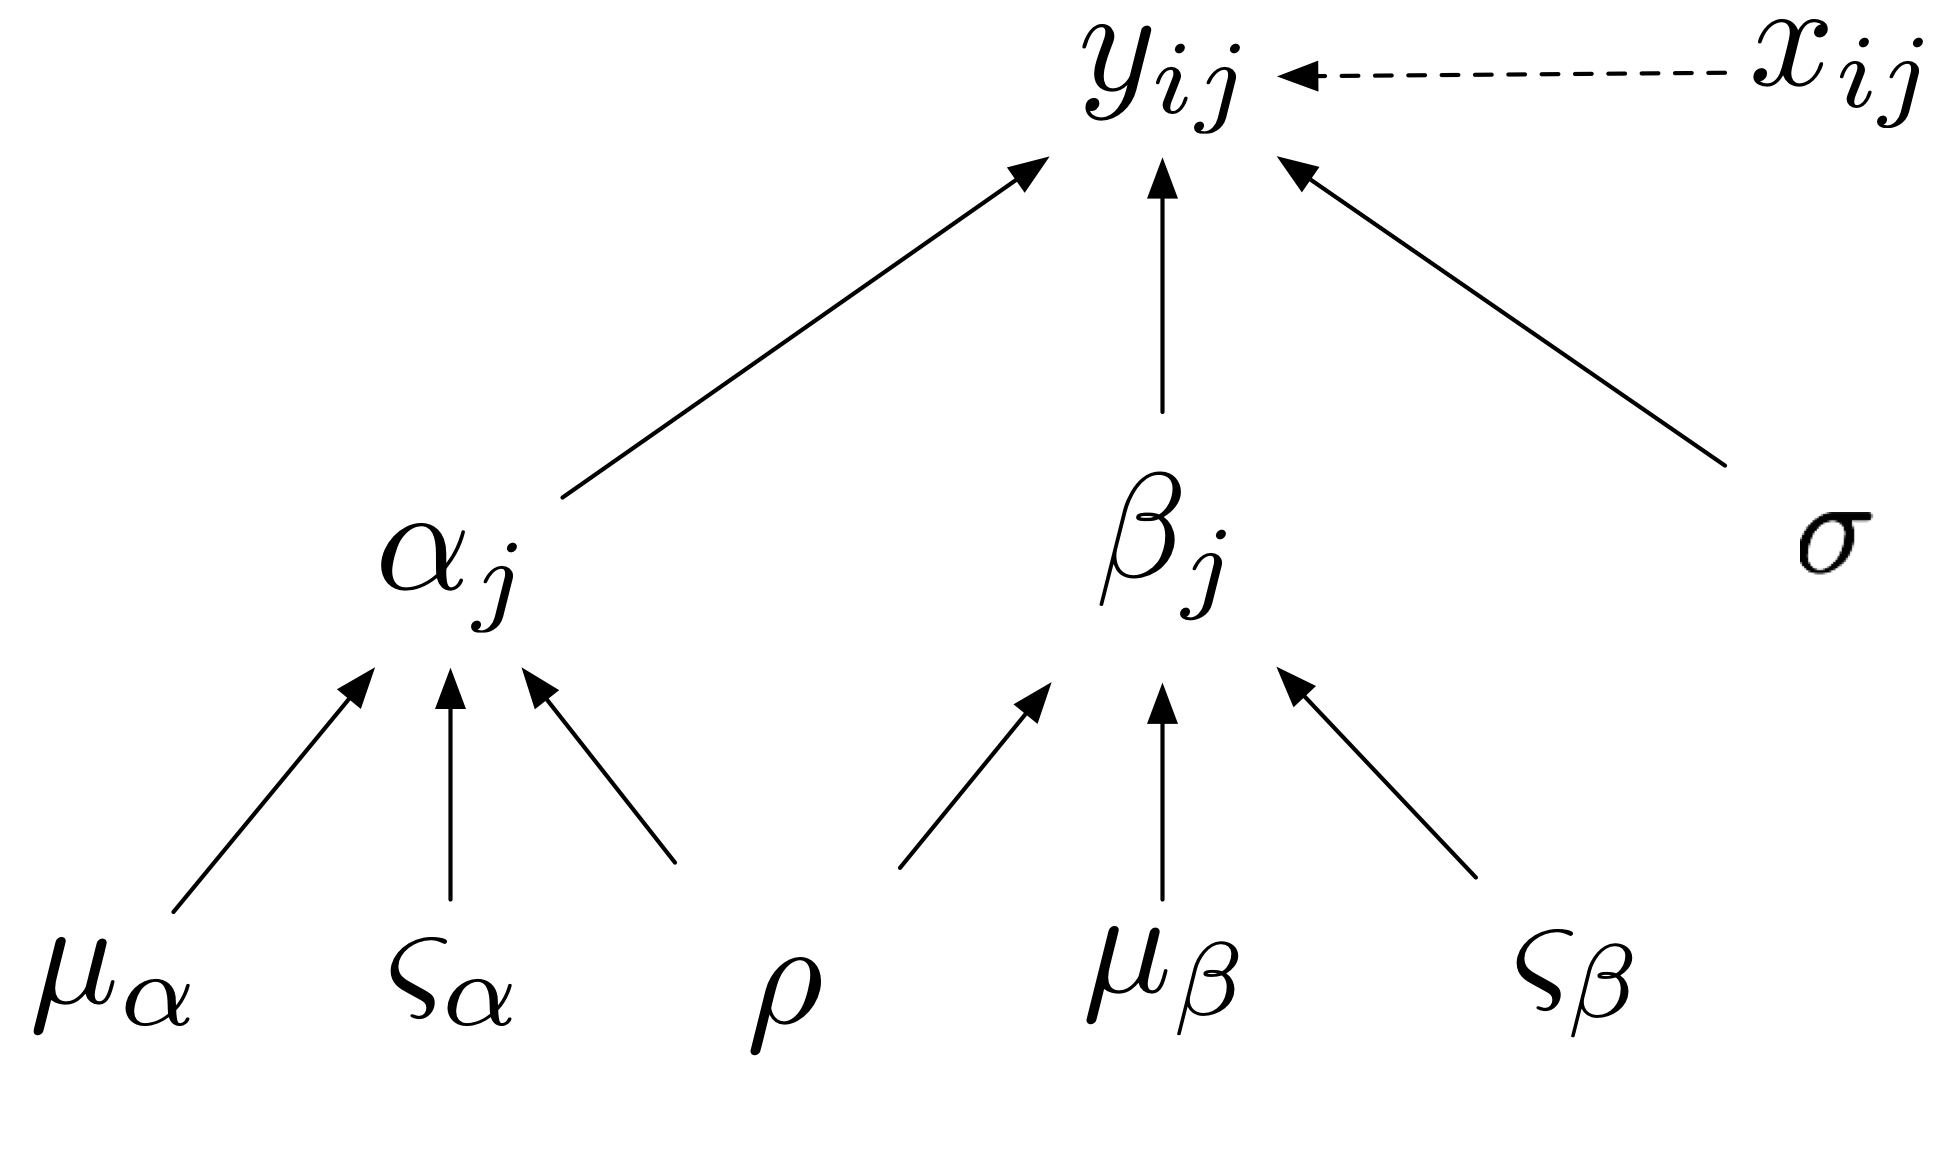
\includegraphics[scale=.5]{DAG5.png}
\end{center}
\begin{align*}
g\big(\alpha_{j},\beta_{j},x_{ij}\big) &=\alpha_{j}+\beta_{j}\log\big(x_{ij}\big)\\
\big[\bm{\alpha},\bm{\beta},\mu_{\alpha},\mu_{\beta},\sigma,\varsigma_{\alpha},\varsigma_{\beta},\rho\mid\mathbf{y}\big] & \propto\prod_{j=1}^{J}\prod_{i=1}^{n_{j}}\text{normal}\big(\log(y_{ij})\mid g\big(\alpha_{j},\beta_{j},x_{ij}\big),\sigma^{2}\big)\nonumber \\
  &\times\text{multivariate normal}\left(\left(\begin{array}{c} \alpha_{j}\\
\beta_{j}
\end{array}\right)\biggm|\left(\begin{array}{c}
\mu_{\alpha}\\
\mu_{\beta}
\end{array}\right),\left(\begin{array}{cc}
\varsigma_{\alpha}^{2} & \rho\varsigma_{\alpha}\varsigma_{\beta}\\
\rho\varsigma_{\alpha}\varsigma_{\beta} & \varsigma_{\beta}^{2}
\end{array}\right)\right)\nonumber \\
 & \times \text{normal}\big(\mu_{\alpha}\mid 0,1000\big)\\
 & \times \text{normal}\big(\mu_{\beta}\mid 0,1000\big)\\
 & \times \text{uniform}\big(\sigma\mid 0,100\big)\\
 & \times \text{uniform}\big(\varsigma_{\alpha}\mid 0,200\big)\\
 & \times \text{uniform}\big(\varsigma_{\beta}\mid 0,200\big) \\
 & \times \text{uniform}\big(\rho \mid 0,1\big)\\
\end{align*}
\fi
 
\section*{References}
\begin{hangparas}{.25in}{1} 
Carey, K. 2007. Modeling $N\textsubscript{2}O$ emission from agricultural soils using a multilevel linear regression. (Doctoral dissertation, Duke University).

\vspace{.5cm}
Qian, S. S., Cuffney, T.  F., Alameddine, I., McMahon, G., \& Reckhow, K. H. 2010. On the application of multilevel modeling in environmental and ecological studies. Ecology, 91(2), 355-361. 
\end{hangparas} 
\end{document}
